\section{Iterative Co-Segmentation and Joint Registration}
\label{sec:segmentation}
如Figure~\ref{fig:iterative-segmentation-registration}所示展示了迭代分割与配准的系统流程。
\begin{figure*}
	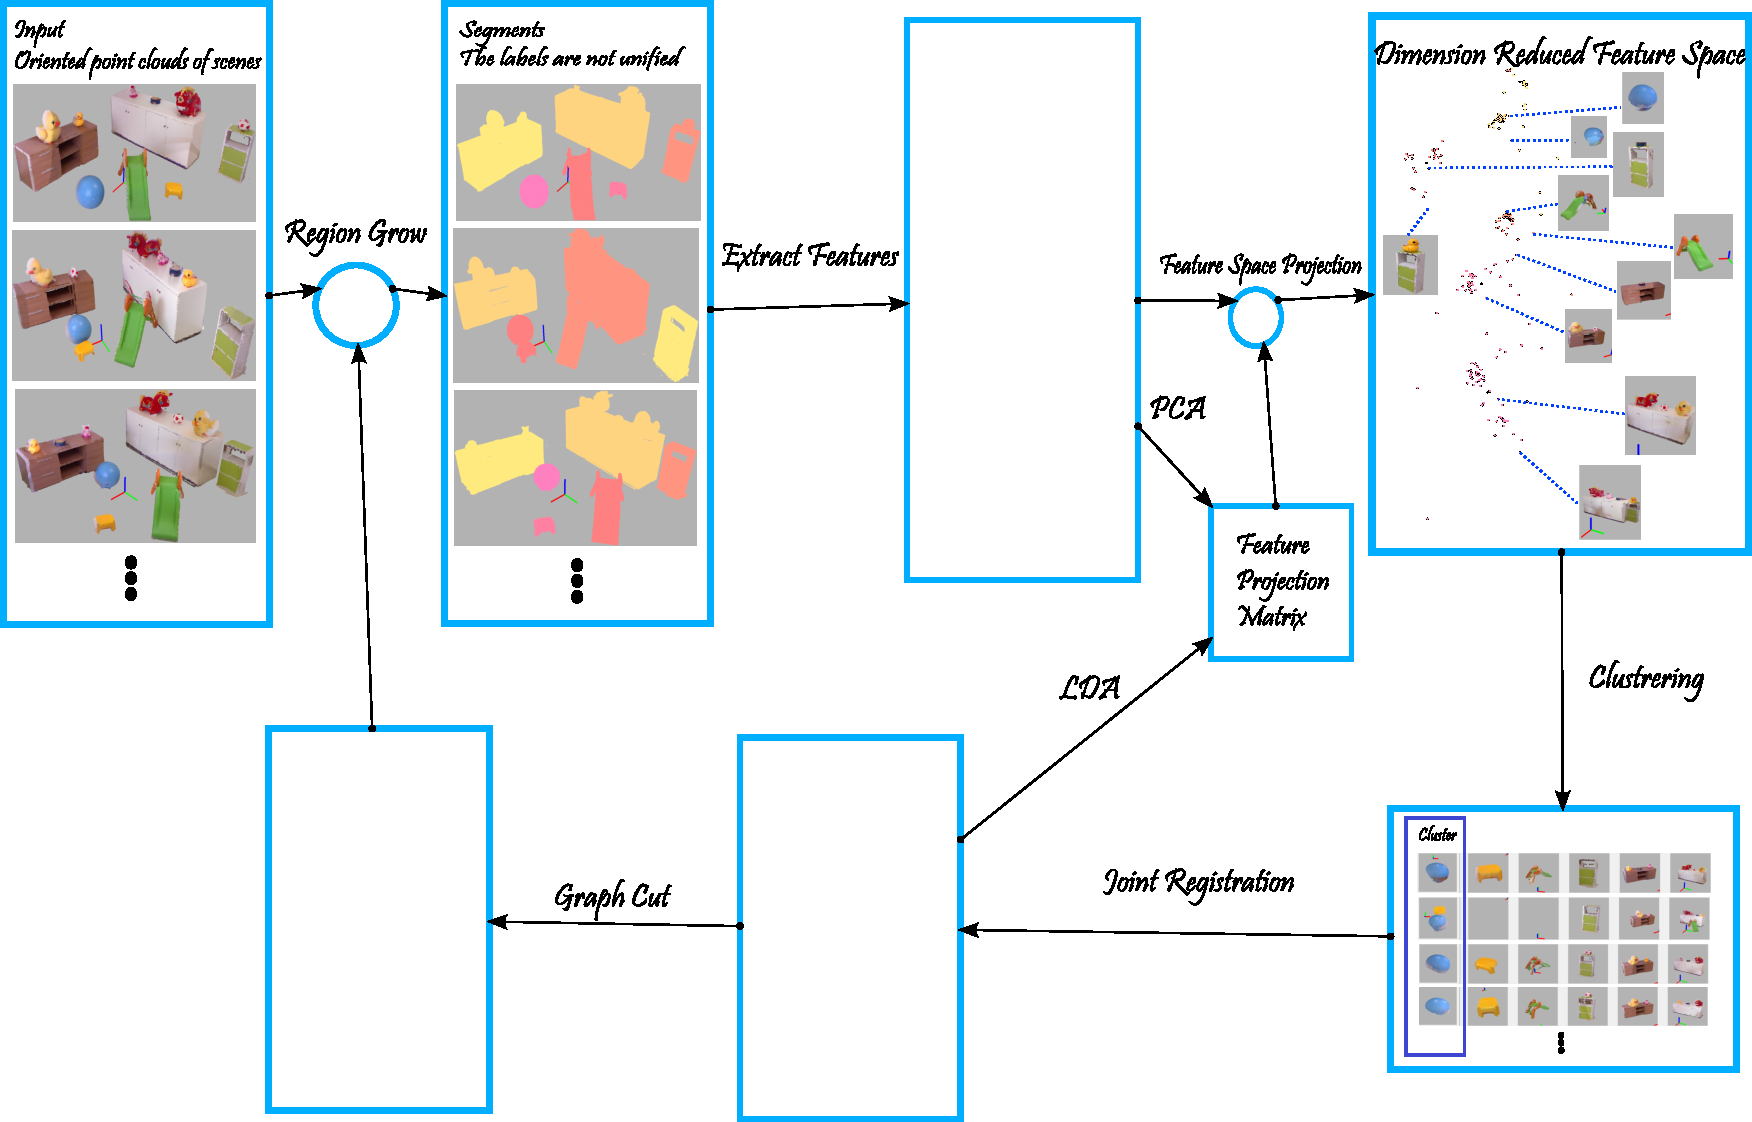
\includegraphics[width=1.0\textwidth]{figures/hsy/overview}
	\caption{Iterative co-segmentation and joint registration.}
	\label{fig:iterative-segmentation-registration}
\end{figure*}
\subsection{Region Grow}
区域生长的操作是对每一帧独立进行的。\\
输入是每一帧的点云以及每一帧所对应的label。\\
输出是更新之后的label。 \\
所谓label就是一个整数的数组它赋予点云中每一个点一个$id$,用来指示它所属的分割区域。我的实现中默认$id=0$的区域是未知区域(在图示中对应黑色区域)。在最开始时label的初始值是全为0。\\
区域生长操作是针对每一帧中的未知区域进行的,所使用的准则是如果两个区域之间有点互相在以R(默认$R=0.02$)为半径的邻域中就将这两个区域合并为同一个区域。\\
选择这样的准则基于的假设是相距较远且不连续的两组点云不太可能属于同一物体。\\
我们认为这样的准则会自然得到欠分割(under-segment)的分割结果。以便于后续能够进行配准(registration)操作\\
\subsection{Object Clustering ( Unify Label )}
这一步操作是将每一帧的不同分割区域的patch无监督的聚成多个类以便于后续对每一类进行配准(registration)。
这一步输入是所有的点云以及它们对应的label,输出仍然是更新之后的label。
先依照前一步的label将点云分成多个patch,对所有的patch提取特征,然后依据投影矩阵将特征降维,然后再在低维空间中根据聚类中心为每一个patch重新分配id并更新每一帧的label。\\
关于使用了哪些特征?\\
如何得到投影矩阵?\\
如何确定聚类中心?\\
以下分别进行说明:
\subsubsection{Features}
Table~\ref{tab:features}列举了所有使用的特征以及对应的维数。
\begin{table}[!hbp]
\begin{tabular}{p{0.73\columnwidth}|{p{0.1\columnwidth}}}
\hline
Feature & Dimension\\
\hline
rgb color histgram & 125\\


\end{tabular}
\caption{Features} %表格的名称
\label{tab:features}
\end{table}
\subsubsection{Projection Matrix}
\subsubsection{Cluster Centers}
\subsection{Joint Registration}
\subsection{Global Consistent Graph Cut}
Figure~\ref{fig:object-iterations} shows the segmentation is progressively refined. 
\begin{figure*}
\centering
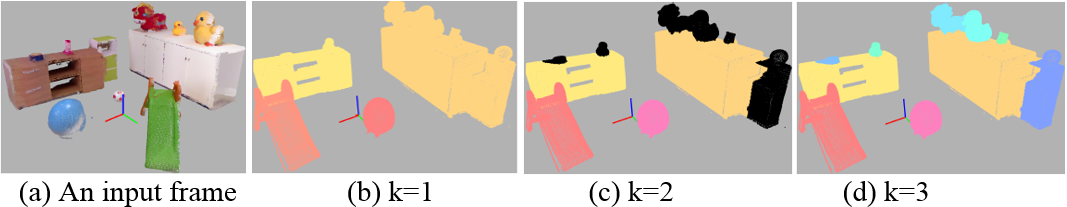
\includegraphics[width=2\columnwidth]{figures/object-iterations.png}
\caption{ The segmentation of each frame is progressively refined based on registered object models. From left to right: an input point cloud (a), segmentation updates at three iterations. \xj{show corresponding object model at each iteration.}}
\label{fig:object-iterations}
\end{figure*}
